\documentclass[11pt]{article}
\usepackage{times}
\usepackage{fullpage}
\usepackage{url}
\usepackage{hyperref}
\usepackage{fancyhdr}
\usepackage{graphicx}
\usepackage{enumitem}
\usepackage{subcaption}
\usepackage{amsmath, amsfonts, amsthm, fouriernc}
\usepackage{IEEEtrantools}
\usepackage{parskip}

\graphicspath{{../chapter/images/}}
\pagestyle{fancy}
\addtolength{\headheight}{2em}
\addtolength{\headsep}{1.5em}
\lhead{\large{ME 2801}}

\usepackage{sectsty}
\sectionfont{\fontsize{12}{8}\selectfont}

\begin{document}

\begin{center}
  \Large{\bf{Assignment: Time Response}}
\end{center}

The textbook exercises, designated with the word ``Nise'', are from the
``Problems'' section at the end of Chapter~4 in \emph{Control System
Engineering} by Norman Nise, 7th edition.

% ---------------------------------------------------------------
\section*{Nise 4.2 and 4.3: Step response of first-order system}

For the MATLAB plots, add annotation (by hand or using the computer) to indicate
the \emph{time constant}~$\tau$ of the system.

% ---------------------------------------------------------------
\section*{Nise 4.8: Pole-zero maps and step responses}

\begin{itemize}
  \item Generate the pole-zero plots by hand; a simple sketch of the $s$-plane
    is sufficient.
    \begin{itemize}
      \item The MATLAB function \texttt{roots()} finds roots of polynomials
        (useful if you want to avoid the quadratic formula).
      \item Optional: \texttt{pzmap()} checks your work directly from the
        transfer function.
    \end{itemize}
  \item Use the MATLAB \texttt{step()} command to plot the step response.
    The goal is to build intuition connecting pole-zero locations to
    time-response character.
  \item The \emph{general forms} referred to in the problem statement are:
    \begin{IEEEeqnarray*}{rCl}
      c(t) & = & K[1-e^{-at}]  \\
      c(t) & = & K[1-Ae^{-\sigma_1 t}-Be^{-\sigma_2 t}] \\
      c(t) & = & K[1-Ae^{-\sigma_d t} \cos(\omega_d t - \phi)] \\
      c(t) & = & K[1 - A \cos(\omega_1 t - \phi)] \\
      c(t) & = & K[1 - Ae^{-\sigma_1 t} - B\,t\,e^{-\sigma_1 t}]
    \end{IEEEeqnarray*}
    Without computing the full inverse Laplace transform, identify numeric
    values for $a$, $\sigma_1$, $\sigma_2$, $\sigma_d$, $\omega_d$, $\omega_1$
    from the appropriate general form.  You do not need to find the coefficients
    $K$, $A$, $B$.
\end{itemize}

% ---------------------------------------------------------------
\section*{Nise 4.20 and 4.21: Response of second-order system}

Parts~(a) and~(b) only.

\subsection*{Nise 4.20: Computing performance metrics}

For calculating rise time~$T_r$ by hand, use the polynomial approximation from
the textbook (footnote~5 to Section~4.6):
\[
  \omega_n T_r \approx 1.76\zeta^3 - 0.417\zeta^2 + 1.039\zeta + 1
  \qquad (0 < \zeta < 0.9,\;\text{error} < 0.5\%)
\]
Alternatively, Figure~4.16 (reproduced below) can be used as a lookup table.

\begin{figure}[h]
  \centering
  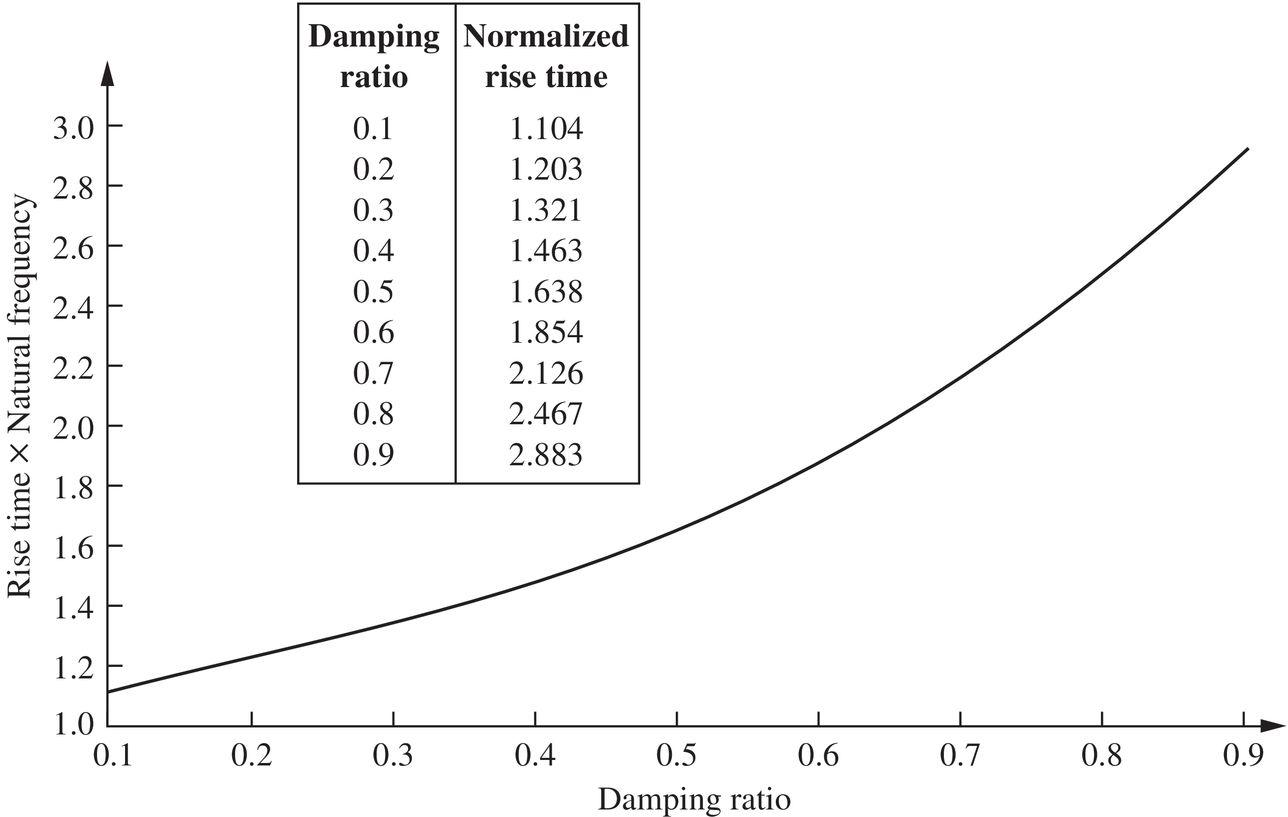
\includegraphics[width=0.7\textwidth]{fig_04_16.jpg}
  \caption{Normalized rise time vs.\ damping ratio for an underdamped
    second-order step response (Nise Fig.~4.16).}
  \label{fig:figure_4_16}
\end{figure}

% ---------------------------------------------------------------
\section*{Nise 4.23: From performance specifications to pole locations}

Given desired transient specifications (\%OS and $T_s$, or \%OS and $T_p$),
find the required pole locations.  This is the \emph{design} direction:
specifications~$\to$ parameters~$\to$ poles.

Use the following relationships:
\begin{align*}
  \zeta   &= \frac{-\ln(\%OS/100)}{\sqrt{\pi^2 + \ln^2(\%OS/100)}} \\[4pt]
  T_p     &= \frac{\pi}{\omega_d} = \frac{\pi}{\omega_n\sqrt{1-\zeta^2}} \\[4pt]
  T_s     &\approx \frac{4}{\zeta\omega_n}
\end{align*}

Use MATLAB to check your answers: build the transfer function from your computed
poles, plot the step response with \texttt{step()}, and verify metrics with
\texttt{stepinfo()}.

% ---------------------------------------------------------------
\section*{Nise 4.32: Step response from pole-zero description}

Check your answers by using MATLAB to plot the step response and verify that
the results agree with the graphs in the exercise.

\end{document}
